% app2.tex (file to switch to appendix mode)

\invisiblechapter{\celloPiece}

\vspace{3.8cm}

\begin{center}

\textsc{for solo violoncello}

\vspace{2.8cm}

\HRule{0.5pt}

\LARGE \textbf{\uppercase{\celloPiece}}

\HRule{2pt}

\vspace{1.8cm}

\normalsize \today

\vspace{3.8cm}

Rhys Gray

\end{center}
\newpage

\section*{Program Notes}
\celloPiece is a piece for solo violoncello, written to explore multiphonics. 

Multiphonics are notated as a harmonic position, with an `M' and the string number (I-IV). 
The theoretical sounding pitches are given in a bracketed staff above the main stave.
String multiphonics are achieved through clusters of close harmonic nodes, and by playing a harmonic close to the highest partial.
To aid the performer during their practice, the sounding partials are given (i.e. M IV [4th + 13th + 9th + 15th + 5th]).
Note that not all of these pitches will actually sound in practice.
The bow should exert slightly more pressure than usual and should be drawn with a consistent speed which should be slower than for harmonics.

\section*{Notation}
\begin{itemize}

    \item Sounding pitch is provided in the stave below.
    \item Multiphonics are denoted with a diamond notehead, marked with an M. Precise tuning in cents (i.e. +41c) is provided to help the performer pitch the multiphonic.
    \item n denotes \emph{normale}.
    \item sp denotes \emph{sul ponticello}.
    \item msp denotes \emph{molto sul ponticello}.
    \item similarly, st denotes \emph{sul tasto}, and mst denotes \emph{molto sul tasto}
\end{itemize}

\newpage
\label{app:to/do Score}
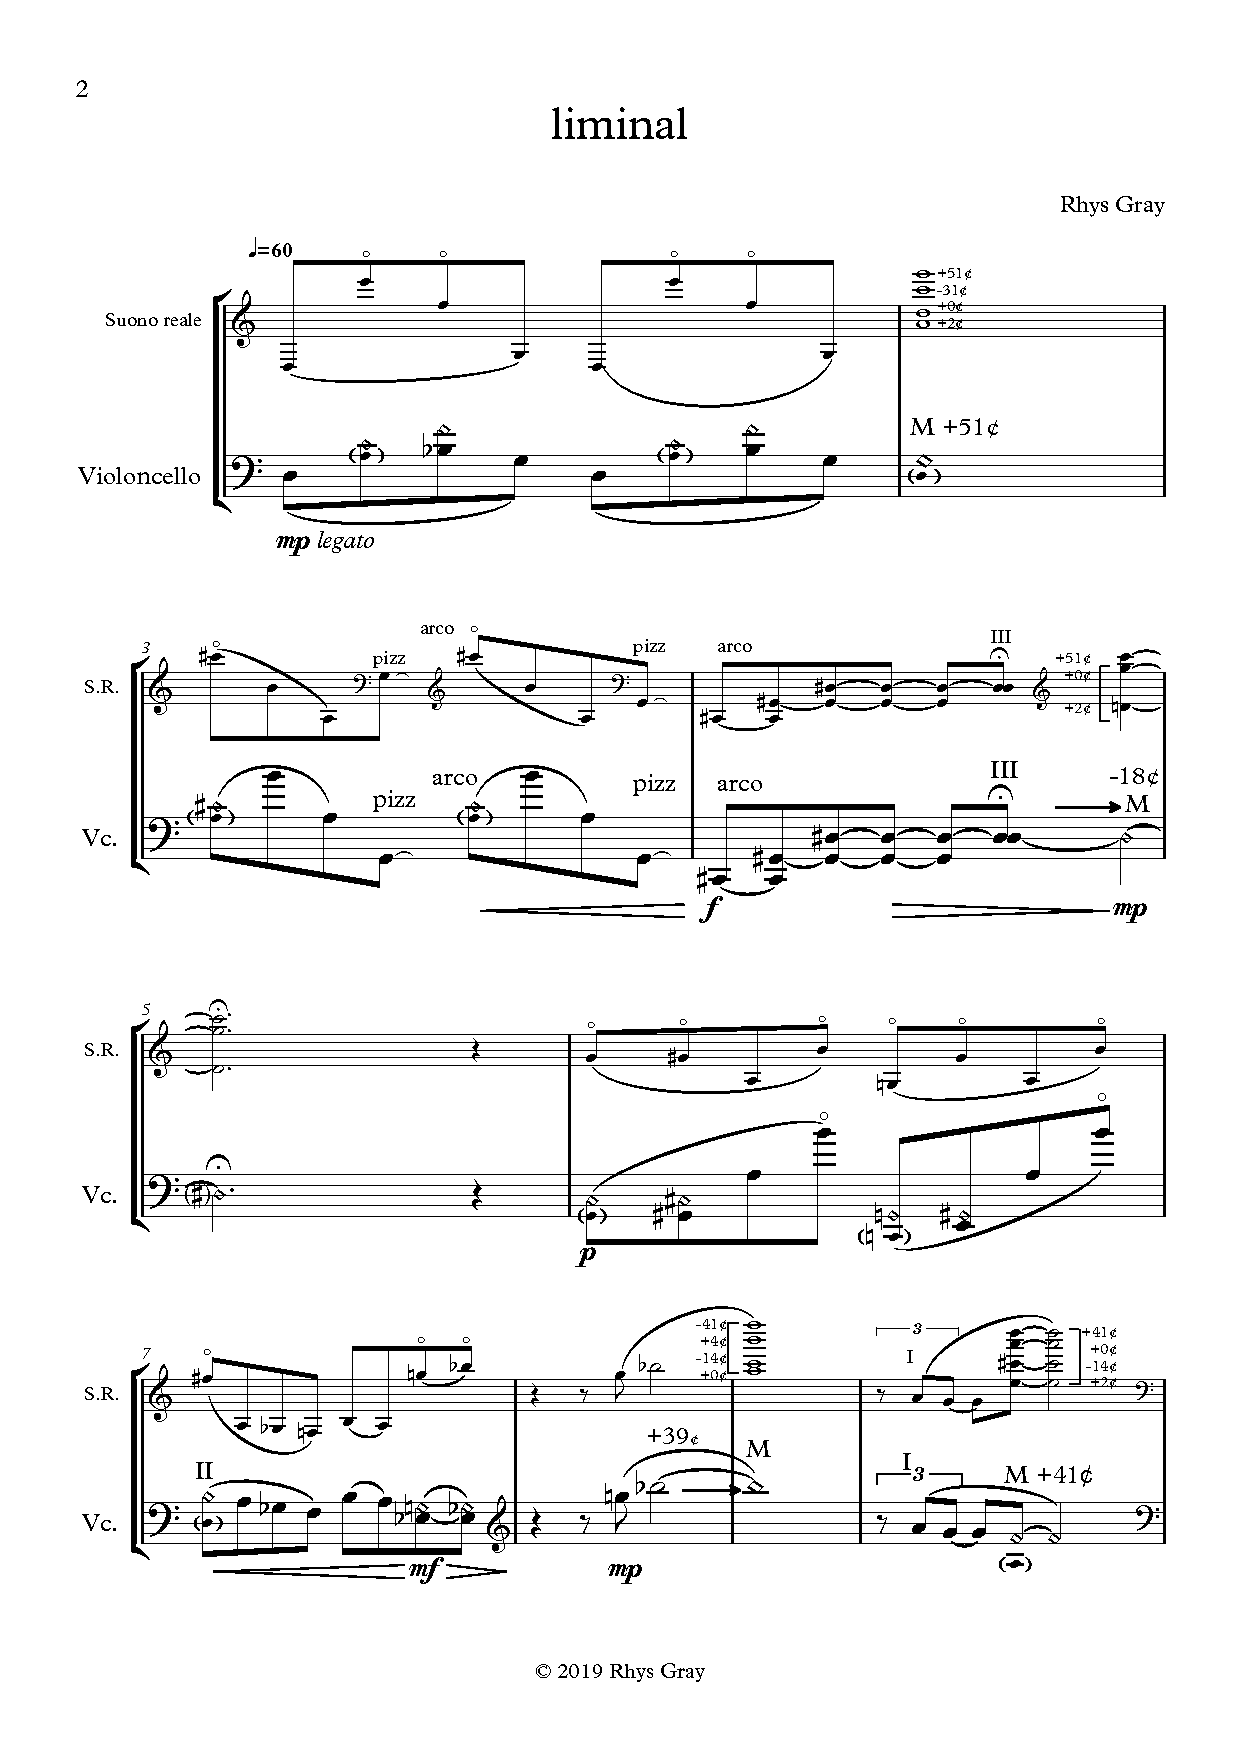
\includepdf[pages=-,pagecommand={}]{resources/compositions/violoncello.pdf}